\documentclass[12pt]{article}
\usepackage[margin=1in]{geometry}
\usepackage{amsthm,amssymb,amsfonts}
\usepackage{tipa}
\usepackage{ gensymb }
\usepackage[fleqn]{amsmath}
\usepackage{dsfont}
\usepackage{graphicx}
 
\newcommand{\N}{\mathbb{N}}
\newcommand{\Z}{\mathbb{Z}}
\newcommand{\dbarl}{\left\lVert}
\newcommand{\dbarr}{\right\rVert}
\newcommand{\sqbrl}{\left[}
\newcommand{\sqbrr}{\right]}
\newcommand{\barl}{\left\lVert}
\newcommand{\barr}{\right\rVert}

\graphicspath{{images/}}

\newenvironment{problem}[2][Problem]{\begin{trivlist}
\item[\hskip \labelsep {\bfseries #1}\hskip \labelsep {\bfseries #2.}]}{\end{trivlist}}
%If you want to title your bold things something different just make another thing exactly like this but replace "problem" with the name of the thing you want, like theorem or lemma or whatever
 
\begin{document}
 
%\renewcommand{\qedsymbol}{\filledbox}
%Good resources for looking up how to do stuff:
%Binary operators: http://www.access2science.com/latex/Binary.html
%General help: http://en.wikibooks.org/wiki/LaTeX/Mathematics
%Or just google stuff
 
\title{MATH 114 - Fall 2016 - Assignment 5}
\author{James Sinn - 20654551}
\maketitle

\begin{problem}{1}
	Inverses
\end{problem}
a) Let A equal the given matrix\\
\[A^{-1} = \sqbrl\begin{array}{ccc|ccc}
1 & 1 & 2 & 1 & 0 & 0\\
1 & 2 & 2 & 0 & 1 & 0 \\
1 & -1 & 3 & 0 & 0 & 1
\end{array}\sqbrr\begin{matrix}\\R_2 - R_1\\R_3 - R_1\end{matrix}\]
\[\sim \sqbrl\begin{array}{ccc|ccc}
1 & 1 & 2 & 1 & 0 & 0\\
0 & 1 & 0 & -1 & 1 & 0\\
0 & -2 & 1 & -1 & 0 & 1
\end{array}\sqbrr\begin{matrix}R_1 - R_2\\\\R_3 + 2R_2\end{matrix}\]
\[\sim \sqbrl\begin{array}{ccc|ccc}
1 & 0 & 2 & 2 & -1 & 0\\
0 & 1 & 0 & -1 & 1 & 0\\
0 & 0 & 1 & -3 & 2 & 1
\end{array}\sqbrr\begin{matrix}R_1 - 2R_3\\\\\end{matrix}\]
\[\sim \sqbrl\begin{array}{ccc|ccc}
1 & 0 & 0  & 8 & -5 & -2\\
0 & 1 & 0 & -1 & 1 & 0\\
0 & 0 & 1 & -3 & 2 & 1
\end{array}\sqbrr\]

\[A^{-1} = \sqbrl\begin{matrix}8 & -5 & -2\\-1 & 1 & 0\\-3 & 2 & 1\end{matrix}\sqbrr\]
b) Let A equal the given matrix\\
\[A^{-1} = \sqbrl\begin{array}{ccc|ccc}
2 & 3 & -1 & 1 & 0 & 0\\
4 & 2 & 1 & 0 & 1 & 0 \\
-2 & 5 & -5 & 0 & 0 & 1
\end{array}\sqbrr\begin{matrix}\\R_2 - 2R_1\\R_3 + R_1\end{matrix}\]
\[A^{-1} = \sqbrl\begin{array}{ccc|ccc}
2 & 3 & -1 & 1 & 0 & 0\\
0 & -4 & 3 & -2 & 1 & 0 \\
0 & 8 & -6 & 1 & 0 & 1
\end{array}\sqbrr\begin{matrix}\\\\R_3 + 2R_2\end{matrix}\]
\[A^{-1} = \sqbrl\begin{array}{ccc|ccc}
2 & 3 & -1 & 1 & 0 & 0\\
0 & -4 & 3 & -2 & 1 & 0 \\
0 & 0 & 0 & -3 & 2 & 1
\end{array}\sqbrr\begin{matrix}\\\\R_3 + 2R_2\end{matrix}\]
Because there is a full row of 0's, the determinant is 0, therefore there is no inverse.

\begin{problem}{2}
	System of Equations
\end{problem}
\[A = \sqbrl\begin{array}{ccc|ccc}
1 & 2 & 2 & 1 & 0 & 0\\
0 & 1 & 2 & 0 & 1 & 0\\
 -1 & 3 & 12 & 0 & 0 & 0\end{array}\sqbrr
\begin{matrix}R_1 - R_2\\\\R_3 - R_1\end{matrix}\]

\[\sim \sqbrl\begin{array}{ccc|ccc}
1 & 1 & 0 & 1 & -1 & 0\\
0 & 1 & 2 & 0 & 1 & 0\\
 -2 & 1 & 10 & -1 & 0 & 1\end{array}\sqbrr
\begin{matrix}\\\\R_3 + 2R_1\end{matrix}\]

\[\sim \sqbrl\begin{array}{ccc|ccc}
1 & 1 & 0 & 1 & -1 & 0\\
0 & 1 & 2 & 0 & 1 & 0\\
 0 & 3 & 10 & 1 & -2 & 1\end{array}\sqbrr
\begin{matrix}\\\\R_3 - 3R_2\end{matrix}\]

\[\sim \sqbrl\begin{array}{ccc|ccc}
1 & 1 & 0 & 1 & -1 & 0\\
0 & 1 & 2 & 0 & 1 & 0\\ 
0 & 0 & 4 & 1 & -5 & 1\end{array}\sqbrr
\begin{matrix}\\\\\frac{1}{4}R_3\end{matrix}\]

\[\sim \sqbrl\begin{array}{ccc|ccc}
1 & 1 & 0 & 1 & -1 & 0\\
0 & 1 & 2 & 0 & 1 & 0\\ 
0 & 0 & 1 & \frac{1}{4} & \frac{-5}{4} & \frac{1}{4}\end{array}\sqbrr
\begin{matrix}R_1 - (R_2 - R_3)\\R_2 - 2R_3\\\end{matrix}\]

\[\sim \sqbrl\begin{array}{ccc|ccc}
1 & 0 & 0 & \frac{3}{2} & \frac{-9}{2} & \frac{1}{2}\\
0 & 1 & 0 & \frac{-1}{2} & \frac{7}{2} & \frac{-1}{2}\\ 
0 & 0 & 1 & \frac{1}{4} & \frac{-5}{4} & \frac{1}{4}\end{array}\sqbrr\]

\[ A^{-1} = \sqbrl\begin{matrix}\frac{3}{2} & \frac{-9}{2} & \frac{1}{2}\\\frac{-1}{2} & \frac{7}{2} & \frac{-1}{2}\\ \frac{1}{4} &\frac{-5}{4} & \frac{1}{4}\end{matrix}\sqbrr\]

\[A^{-1}\vec{b} = \vec{x}\]

\[\sqbrl\begin{matrix}\frac{3}{2} & \frac{-9}{2} & \frac{1}{2}\\\frac{-1}{2} & \frac{7}{2} & \frac{-1}{2}\\ \frac{1}{4} &\frac{-5}{4} & \frac{1}{4}\end{matrix}\sqbrr\sqbrl\begin{matrix}b_1\\b_2\\b_3\end{matrix}\sqbrr = \begin{matrix}\frac{3}{2}b_1 - \frac{9}{2}b_2 + \frac{1}{2}b_3 = x_1\\
\frac{-1}{2}b_1 + \frac{7}{2}b_2 - \frac{1}{2}b_3 = x_2\\
\frac{1}{4}b_1 - \frac{5}{4}b_2 + \frac{1}{4}b_3 = x_3\end{matrix}\]


\begin{problem}{3}
	Theory/Proofs
\end{problem}
I worked through this but couldn't figure it out.\\
\begin{problem}{4}
\end{problem}
Yes, this is because if there are any rows with 0's, then it is non invertible, meaning that the rank must be equal to each other.\\

\begin{problem}{5}
\end{problem}
I couldn't figure out how to prove this.\\

\begin{problem}{6}
	Determinants
\end{problem}
a) Let A equal the given matrix.\\
\[det(A) = 1(39 - 21) + 2(15-9) + 3(-35 + 39)\]
\[= 18 + 12 + 12 = 42\]
A is invertible because det(A) is not 0.\\

b) Let A equal the given matrix.\\
\[det(A) = 2((det\left(\sqbrl\begin{matrix}-7 & -5 & 0\\8 & 6 & 0\\ 7 & 5 & 4\end{matrix}\sqbrr\right)
			+ det\left(\sqbrl\begin{matrix} 0 & 0 & 8\\-7&-5&0\\7&5&4\end{matrix}\sqbrr\right)
			+ 3det\left(\sqbrl\begin{matrix}0 & 0 & 8\\-7 & -5 & 0\\7&5&4\end{matrix}\sqbrr\right)\]

\[= 2( -7(24 -5) + 8(-20 -5)) + (8(0 - 40) + 7( 0 -48)) + 3(-7(0-40) + 7(0+40)) = 358\]
Since det(A) is not equal to 0, the matrix A is invertible.\\\\

c) Let A equal the given matrix.\\
For the record, this is a horrible thing to do to someone if they didn't know about the rules.
Matrix A is not invertible, as the determinant is 0.\\
This can also be proven because rank(A) is not equal to 5, it is instead 4, if the matrix were invertible, it would have to be equal to $n$

\begin{problem}{7}
\end{problem}
For what values of $s$ make the below matrix invertible.
\[A = \sqbrl\begin{matrix}1 & s & 1\\s & -3 & -2s\\1 & 2 & -1\end{matrix}\sqbrr\]
For this to be invertible, the determinant must not be 0. Because of this, we can solve for s. (it should be a quadratic.)\\
\[det(A) = 1(3 - 4s) + s(-s -2) + 1 (-s -2) = 3 - 4s + -s^2 -2s -s -2\]
\[= -s^2 -7s + 1\]
\[ s = \frac{1}{2}(\sqrt{53} -7)\]
\[ s = \frac{1}{2}(-\sqrt{53} -7)\]
This means that for all values of s, where s is a real number, and provided s is not one of the above two values the matrix is invertible.\\

\begin{problem}{8}
\end{problem}
Let matrix A equal the given matrix.\\
\[det(A) = (1+i)(3-i) - (1+3i)(1-i)\]
\[= (3 - i + 3i +1) - (1 - i + 3i +3)\]
\[= (2i + 4) - (2i + 4) = 0\]
Because det(A) is 0, A is not invertible.\\

\begin{problem}{9}
\end{problem}
\[A = \sqbrl\begin{matrix}a_{11} & a_{12} & a_{13}\\a_{21} & a_{22} & a_{23}\\a_{31} & a_{32} & a_{33}\end{matrix}\sqbrr\]
\[A^T = \sqbrl\begin{matrix}a_{11} & a_{21} & a_{31}\\a_{12} & a_{22} & a_{32}\\a_{13} & a_{23} & a_{33}\end{matrix}\sqbrr\]

\[det(A) = a_{11}(a_{22}a_{33} - a_{32}a_{23}) + a_{21}(a_{12}a_{23} - a_{32}a_{33}) + a_{31}(a_{12}a_{23} - a_{22}a_{23})\]
\[det(A^T) = a_{11}(a_{22}a_{33} - a_{32}a_{23}) + a_{21}(a_{12}a_{23} - a_{32}a_{33}) + a_{31}(a_{12}a_{23} - a_{22}a_{23})\]

Both determinants are indeed the same, and it does generalize to an $n\times n$ matrix. This is because when transposing a matrix, and then changing to do cofactor expansion on the first row instead of first column, you are effectively transposing the operation too, causing the result to be the exact same.

\begin{problem}{10}
\end{problem}
a)\\
\[det(A)det(B) = 6\]
\[det(B)det(C) = 12\]
\[det(A)det(B)det(C) = 24\]
\[det(B) = ?\]
\[\frac{det(A)det(B)det(C)}{det(B)det(C)} = 2 = det(A)\]
\[\frac{det(A)det(B)}{det(A)} = 3\]
\[det(B) = 3\]
b)\\
The only two possible values for the determinant of A are 0 and 1. This is because the two matrices that satisfy $A^3 = A$ are the zero matrix, and the identity matrix. Identity matrix has a determinant of 1, and the zero matrix of 0.\\
c)\\
The determinant of an orthogonal matrix ($A^T$) must be either 1 or -1. This is proven by the relationship of determinants of transposed matrices and how they must be equal. To make a bit more mathematical sense. $det(AA^T) = det(A)^2 = det(I) = 1$. This is because $\sqrt{1} = \pm 1$
d)\\


\begin{problem}{11}
	Eigenvalues and Eigenvectors
\end{problem}
a)\\
\[A\vec{v_1} = \sqbrl\begin{matrix}2\\0\end{matrix}\sqbrr\]
\[A\vec{v_2} = \sqbrl\begin{matrix}0\\3\end{matrix}\sqbrr\]
\[A\vec{v_3} = \sqbrl\begin{matrix}2\\3\end{matrix}\sqbrr\]
b)\\
Blue is the input vector, and red is the output vector.\\
\[A\vec{v_1} \]
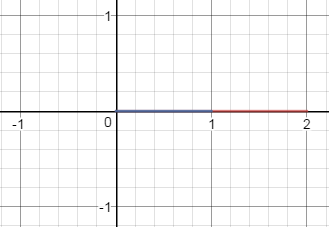
\includegraphics{Av1}

\[A\vec{v_2} \]
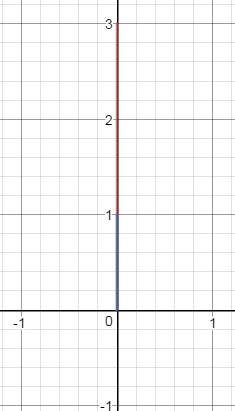
\includegraphics{Av2}

\[A\vec{v_3} \]
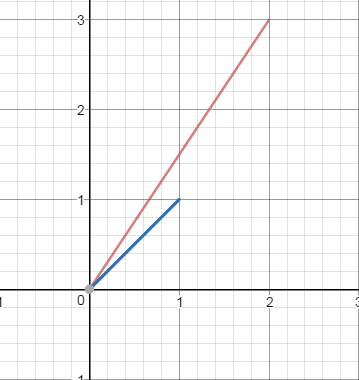
\includegraphics{Av3}\\
c)\\

\begin{problem}{12}
\end{problem}
a)\\
\[\lambda_1 = 3\]
\[\lambda_2 = 1\]

b)\\
\[\lambda_1 = 0\]
\[\lambda_2 = 1\]
\[\lambda_3 = 2\]

\end{document}

